\documentclass{scrbook}
\usepackage{graphicx} % Required for inserting images
\usepackage{tabularx} % Required for fixed width tables
\usepackage{scrlayer-scrpage} % Required for the subtitles
\usepackage{url} % Required for the URLs
\usepackage{hyperref} % Required for the URLs
\usepackage{listings} % Required for the code snippets
\usepackage{mathtools} % Required for the system of equations
\usepackage{amsmath,amssymb} % Required for some math symbols
\usepackage{enumitem} % Required for lettered lists

% Put the caption of the snippets at the bottom
\lstset{
    captionpos=b,
    basicstyle=\ttfamily,
    columns=fullflexible,
    literate={--}{{-}{-}}2
}


\title{Ethereum Virtual Machine}
\subtitle{Ambient intelligence course (A.Y. 2025/2026)\\Topic taught by Prof. Arnaldo Tomasino}
\author{Gabriele Colapinto}
\date{\today}

\begin{document}

\maketitle
\thispagestyle{empty}

{\Large\textbf{License}} \\
{Notes from Ambient intelligence (A.Y. 2025/2026) by Gabriele Colapinto. 
Course taught by professors Michele Ruta, Floriano Scioscia, Arnaldo Tomasino, Davide Loconte — 
Licensed under CC BY-NC 4.0.\\
\url{https://creativecommons.org/licenses/by-nc/4.0/}}

\vspace*{\fill}
\rule{\textwidth}{0.2pt}
\small{© 2025 Gabriele Colapinto \\
Released under the \href{https://creativecommons.org/licenses/by-nc/4.0/}{Creative Commons Attribution–NonCommercial 4.0 International License}}

\clearpage

\tableofcontents

\chapter{The Ethereum Virtual Machine (EVM)}

The Ethereum Virtual Machine (EVM) is the core computational engine of the Ethereum network. It is the environment where all smart contracts are deployed and all transactions are executed. This section deconstructs the EVM's architecture, execution model, and security principles, providing a foundational understanding of how decentralized applications function in a trustless environment.

\section{Core Concepts and Architecture}

The EVM can be defined in several ways, each highlighting a different aspect of its function:

\begin{itemize}
    \item It is a \textbf{consensus-based, globally executed virtual machine}, meaning every full node in the network runs the EVM to validate transactions and maintain consensus.
    
    \item It is a \textbf{formal model of a virtual state machine} that specifies exactly how the Ethereum system state is altered by each transaction.
    
    \item It is the part of Ethereum that specifically \textbf{handles smart contract deployment and execution}.
\end{itemize}

From a practical perspective, the EVM can be conceptualized as a large, decentralized computer. However, its execution environment is fundamentally "lifeless," meaning the global state remains static until a transaction triggers a state transition.

\subsection{State, Accounts, and Transactions}

The Ethereum state is comprised of accounts. There are two distinct types of accounts:

\begin{itemize}
    \item \textbf{Externally Owned Account (EOA):} This account is controlled by a private key held by a user. EOAs are used to initiate transactions, such as sending Ether or interacting with smart contracts.
    
    \item \textbf{Contract Account:} This account is controlled by its own code and possesses an internal, persistent storage. It is activated when it receives a transaction or a message from another contract.
\end{itemize}

When a transaction is sent from an EOA, its effect depends on the destination. If the destination is another EOA, the transaction may simply transfer Ether. If the destination is a contract account, the contract's code is activated and executed. This code can:

\begin{itemize}
    \item Read the contents of the received message.
    \item Read and write to its own internal storage.
    \item Send messages to other contracts, triggering their execution in turn.
\end{itemize}

\subsection{The "Quasi-Turing-Complete" Nature of the EVM}

The EVM is described as "quasi-Turing-complete" rather than fully Turing-complete. This distinction is critical: while high-level smart contract languages like Solidity are designed to be Turing-complete (capable of expressing any computable function, including infinite loops), the EVM's execution environment imposes a hard constraint on all computation: \textbf{gas}. Every operation requires a fee, paid in gas, from a finite pool allocated by the transaction. This mechanism makes infinite loops prohibitively expensive and guarantees that all program executions eventually terminate, ensuring the EVM's deterministic nature.

\section{The Role and Functionality of Smart Contracts}

Smart contracts are the primary application unit on Ethereum. They are autonomous pieces of code that live on the blockchain and can serve several distinct purposes.

\begin{itemize}
    \item \textbf{Data Store:} A contract can maintain a persistent data store, acting as a public database that is useful to other contracts or external applications.
    
    \item \textbf{Forwarder Contract:} A contract can function as an EOA with more complex access policies. For example, a multisignature wallet is a forwarder contract that only forwards a message after receiving approval from a required number of private keys.
    
    \item \textbf{Relationship Management:} Contracts can manage ongoing relationships between users. A common example is a bounty contract that automatically pays a reward to any user who submits a valid solution to a specified problem.
    
    \item \textbf{Software Library:} A contract can provide a set of functions that other contracts can call, serving as a reusable software library on the blockchain.
\end{itemize}

Contracts interact with each other by sending \textbf{messages}. These are similar to transactions but are generated by contracts rather than EOAs. Like transactions, messages that trigger computation also consume gas.

\section{EVM Execution Environment}

The EVM is a \textbf{stack-based virtual machine}. It operates on an instruction set of approximately 140 unique opcodes, each of which manipulates data within specific memory areas. Opcodes are \textbf{1 B} long (two hexadecimal digits) and each one of them has a \textbf{cost}.

\subsection{Memory Areas: Stack, Memory, and Storage}

A smart contract has access to three distinct memory areas during execution, each with unique characteristics and costs. These memory areas are listed in table \ref{tbl:memory_areas}.

\begin{table}[h!]
    \centering
    \begin{tabularx}{\linewidth}{|p{0.25\textwidth}|X|X|}
        \hline
        Area & Characteristics & Purpose\\ \hline
        
        \textbf{Stack} & Max size of 1024 items; each item is a 256-bit word. & Used by instructions to store operands and pass values to functions.\\ \hline
        
        \textbf{Working Memory} & Linear array of bytes; volatile (cleared after execution). & Used for storing local function variables. \\ \hline
        
        \textbf{Storage} & Persistent key-value store (256-bit keys and values); publicly readable; writing is very expensive compared to working memory. & Used to persist information between different smart contract calls.\\ \hline
    \end{tabularx}
    \caption{Memory areas with related characteristics and purpose}
    \label{tbl:memory_areas}
\end{table}

\subsection{The EVM Instruction Set (Opcodes)}

\begin{figure}
    \centering
    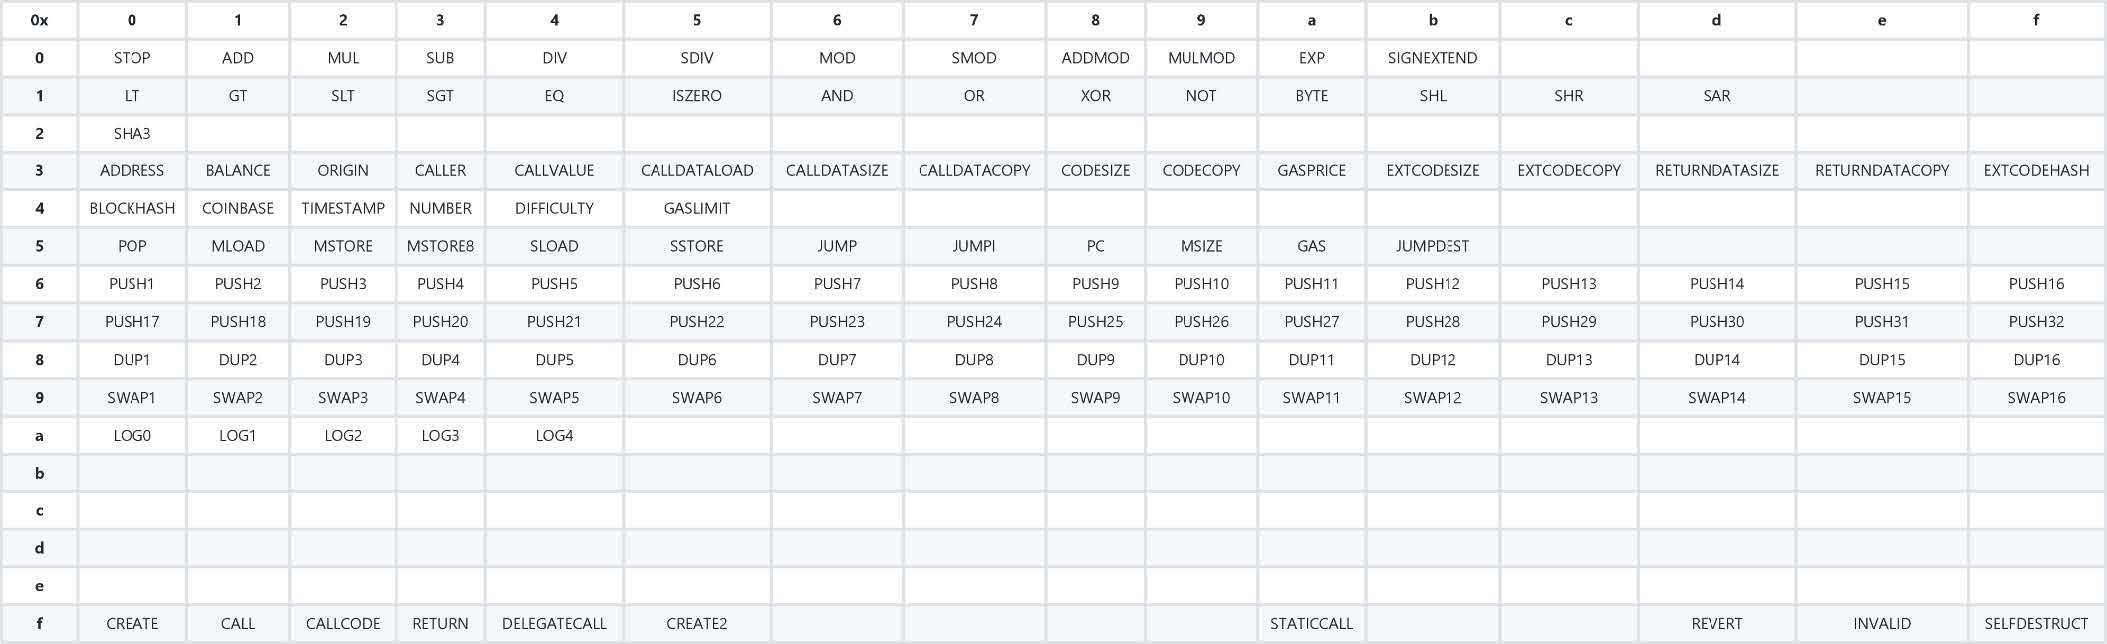
\includegraphics[width=\linewidth]{Images/Instruction_set.jpg}
    \caption{EVM instruction set -- The number of the row corresponds to the first hexadecimal digit of the opcode and the number of the column to its second digit. In fact, \texttt{0x60} $\longrightarrow$ \texttt{PUSH1}.}
    \label{fig:instruction_set}
\end{figure}

EVM instructions, or opcodes, can be grouped into several categories: Stack manipulation, Memory/Storage manipulation, Arithmetic/comparison/bitwise, Program counter related, Environment related, and Halting.\\

Table \ref{tbl:opcodes} shows a few examples of common opcodes and figure \ref{fig:instruction_set} shows a table associating opcodes to their mnemonic counterpart. The reader is encouraged to check the \href{https://www.evm.codes/}{official EVM instruction set web page}.

\begin{table}[h!]
    \centering
    \begin{tabularx}{\linewidth}{|p{0.18\linewidth}|p{0.30\linewidth}|X|}
        \hline
        \textbf{Mnemonic} & \textbf{Opcode Category} & \textbf{Description} \\ \hline
        
        \texttt{POP}, \texttt{PUSHn}, \texttt{DUPn}, \texttt{SWAPn} 
        & Stack Manipulation 
        & Remove, insert, duplicate, or reorder elements on the stack. \\ \hline
        
        \texttt{MLOAD}, \texttt{MSTORE}, \texttt{MSTORE8}, \texttt{MSIZE} 
        & Memory Manipulation 
        & Load from or store data into temporary memory; query memory size. \\ \hline
        
        \texttt{SLOAD}, \texttt{SSTORE} 
        & Storage Manipulation 
        & Load from or store data into persistent contract storage. \\ \hline
        
        \texttt{ADD}, \texttt{SUB}, \texttt{MUL}, \texttt{DIV}, \texttt{MOD}, \texttt{LT}, \texttt{GT}, \texttt{AND}, \texttt{OR} 
        & Arithmetic / Comparison / Bitwise 
        & Perform arithmetic operations, comparisons, and bitwise logic on stack values. \\ \hline
        
        \texttt{JUMP}, \texttt{JUMPI} (jump if, conditional jump), \texttt{PC}, \texttt{JUMPDEST} 
        & Program Counter Related 
        & Modify or inspect the program counter and control execution flow. \\ \hline
        
        \texttt{ADDRESS}, \texttt{CALLER}, \texttt{CALLVALUE}, \texttt{NUMBER} 
        & Environment Related 
        & Access information about the execution environment and transaction context. \\ \hline
        
        \texttt{STOP}, \texttt{RETURN}, \texttt{REVERT}, \texttt{INVALID}, \texttt{SELFDESTRUCT} 
        & Halting 
        & Terminate execution, optionally returning data or reverting state changes. \\ \hline
        
    \end{tabularx}
    \caption{EVM opcodes grouped by category with representative examples}
    \label{tbl:opcodes}
\end{table}

\subsubsection{Stack Semantics and Memory Interaction}

In the EVM, each instruction interacts with the stack in a well-defined way. This behavior can be formally described using two parameters:

\begin{itemize}
    \item $\delta$: the number of items removed (popped) from the stack
    \item $\alpha$: the number of items added (pushed) onto the stack
\end{itemize}

Each opcode consumes $\delta$ elements from the top of the stack and produces $\alpha$ new elements, following a last-in, first-out (LIFO) paradigm.

\paragraph{Stack manipulation instructions}
These instructions directly modify the structure of the stack without performing computations.

\begin{itemize}
    \item \texttt{POP} $(\delta = 1, \alpha = 0)$: removes the top element from the stack.
    \item \texttt{PUSHn} $(\delta = 0, \alpha = 1)$: pushes an immediate value of $n$ bytes onto the stack.
    \item \texttt{DUPn}: duplicates the $n$-th stack element and pushes it on top.
    \item \texttt{SWAPn}: swaps the top element with the $n$-th element below it.
\end{itemize}

\paragraph{Arithmetic instructions}
These instructions consume operands from the stack and push the result back.

\begin{itemize}
    \item \texttt{ADD}, \texttt{SUB} $(\delta = 2, \alpha = 1)$: pop two operands and push the result.
\end{itemize}

\paragraph{Memory interaction}
Some instructions interact with the EVM memory, which is a temporary, byte-addressable, and non-persistent data area.

\begin{itemize}
    \item \texttt{MLOAD} $(\delta = 1, \alpha = 1)$: pops a memory address from the stack, reads 32 bytes (one word) from memory at that address, and pushes the value onto the stack.
    
    \item \texttt{MSTORE} $(\delta = 2, \alpha = 0)$: pops a memory address and a value from the stack, and stores the value (32 bytes) at the specified memory location.
\end{itemize}

\paragraph{Execution model}
The EVM is a stack-based machine: all computations are performed using stack operands. Memory is not accessed directly by instructions, but only indirectly through stack values that represent memory addresses.

For example, the instruction \texttt{MSTORE} does not contain explicit operands. Instead, it expects the required inputs (address and value) to be already present on the stack. This design makes the instruction set compact but requires careful tracking of stack state during execution.

\paragraph{Note on memory}
The EVM memory is sometimes informally compared to a heap, but it differs from traditional heap memory in conventional programming languages:

\begin{itemize}
    \item it is linearly addressed and byte-oriented;
    \item it is reset for every transaction execution;
    \item it is not persistent (unlike storage);
    \item it automatically expands when accessed, incurring additional gas costs.
\end{itemize}

Therefore, instructions such as \texttt{MLOAD} and \texttt{MSTORE} provide the only interface between the stack and this temporary memory space.

\section{The Gas Mechanism: Fueling the EVM}

The gas mechanism is a critical feature of the EVM, designed to prevent Denial of Service (DoS) attacks and resource abuse by assigning a cost to every computational step. Every operation executed inside the EVM is performed by every full node in the network, as required by Ethereum's consensus model.\\

This design provides an important benefit: any smart contract can interact with any other contract without the overhead of external remote procedure calls. However, the drawback is that computation on the EVM is expensive, since it must be replicated across the entire network. As a rule of thumb, one should avoid performing on-chain computations that could be done more efficiently off-chain.\\

Every transaction must include two gas-related fields:

\begin{itemize}
    \item \texttt{GASPRICE}: The fee (in wei, a small denomination of Ether) the sender is willing to pay per unit of gas. Transaction senders are incentivized to choose a reasonable \texttt{GASPRICE}, since values that are too low may lead validators (or miners, in legacy systems) to ignore the transaction.
    
    \item \texttt{STARTGAS}: The total amount of gas allocated for the transaction's execution.
\end{itemize}

When a transaction is processed, the sender must be able to afford the maximum possible cost. Therefore, an amount equal to \texttt{STARTGAS * GASPRICE}, together with the transferred value, is reserved (or effectively deducted) from the sender's account balance before execution begins.\\

The process of calculating the gas cost for a transaction is as follows:

\begin{itemize}
    \item The initial gas available for computation is \texttt{STARTGAS} minus a base fee of 21,000 gas. An additional fee is subtracted based on the transaction's data size (for example, earlier versions of the protocol charged 68 gas per non-zero byte, later reduced to 16).
    
    \item For each instruction executed by the EVM, a specific amount of gas is subtracted from the remaining total, according to the cost of the corresponding opcode and possible dynamic factors such as memory expansion.
    
    \item If the execution completes successfully with \texttt{N >= 0} gas remaining, the sender is refunded an amount equal to \texttt{N * GASPRICE} in wei.
    
    \item If execution runs out of gas or fails, all state changes are reverted, but the gas consumed up to that point is not refunded.
\end{itemize}

The cost of most instructions falls into one of several groups listed in table \ref{tbl:instruction_costs_group}.\\

\begin{table}[h!]
    \centering
    \begin{tabularx}{\linewidth}{|p{0.18\linewidth}|p{0.15\linewidth}|X|}
        \hline
        \textbf{Group} & \textbf{Gas Cost} & \textbf{Examples and Description} \\ \hline
        
        \texttt{Gzero} & 0 
        & \texttt{STOP}, \texttt{RETURN} --- Instructions that terminate execution without additional computational cost. \\ \hline
        
        \texttt{Gbase} & 2 
        & \texttt{ADDRESS}, \texttt{POP}, \texttt{PC} --- Simple operations with minimal computational effort. \\ \hline
        
        \texttt{Gverylow} & 3 
        & \texttt{ADD}, \texttt{SUB}, \texttt{LT}, \texttt{AND}, \texttt{MLOAD}, \texttt{MSTORE} --- Basic arithmetic, logical, and memory operations. \\ \hline
        
        \texttt{Glow} & 5 
        & \texttt{MUL}, \texttt{DIV}, \texttt{SDIV}, \texttt{MOD} --- More expensive arithmetic operations. \\ \hline
        
        \texttt{Gmid} & 8 
        & \texttt{ADDMOD}, \texttt{MULMOD}, \texttt{JUMP} --- Medium-cost operations, including modular arithmetic and control flow changes. \\ \hline
        
        \texttt{Ghigh} & 10 
        & \texttt{JUMPI} --- Higher-cost conditional control flow operations. \\ \hline
        
    \end{tabularx}
    \caption{EVM instruction gas cost groups with representative examples}
    \label{tbl:instruction_costs_group}
\end{table}

\noindent
\textit{Note:} The values reported in table \ref{tbl:instruction_costs_group} refer to the base cost of instructions. 
The actual gas cost may vary depending on the execution context, for example due to memory expansion, storage access (e.g., \texttt{SLOAD}, \texttt{SSTORE}), or other dynamic factors such as operands length (for example, the instruction \texttt{SHA3} costs 30 gas + 6 gas per word).

\section{The EVM Security Model}

The EVM is a security-oriented virtual machine designed to operate in a global, adversarial environment. Its security is enforced through four key restrictions:

\begin{enumerate}
    \item \textbf{Paid Computation:} Every computational step must be paid for upfront through the gas mechanism. This prevents malicious actors from bogging down the network with resource-intensive, non-terminating programs.
    
    \item \textbf{Sandboxed Execution:} A contract is executed in a sandbox. It may only access and modify its own internal state or trigger the execution of other contracts. It cannot affect anything else on the node's machine.
    
    \item \textbf{Isolated State:} Contracts cannot directly access or read each other's state (storage). They may only interact by transmitting a single, arbitrary-length byte array as a message.
    
    \item \textbf{Deterministic Execution:} Program execution is fully deterministic. For any given starting state and transaction, every conforming EVM implementation will produce an identical final state. This is essential for achieving network-wide consensus.
\end{enumerate}

\section{Practical Example: EVM Bytecode Execution}

To understand how these concepts come together, we can examine the execution of simple EVM bytecode.

\subsection{Example 1: Summing Two Values}

\begin{figure}
    \centering
    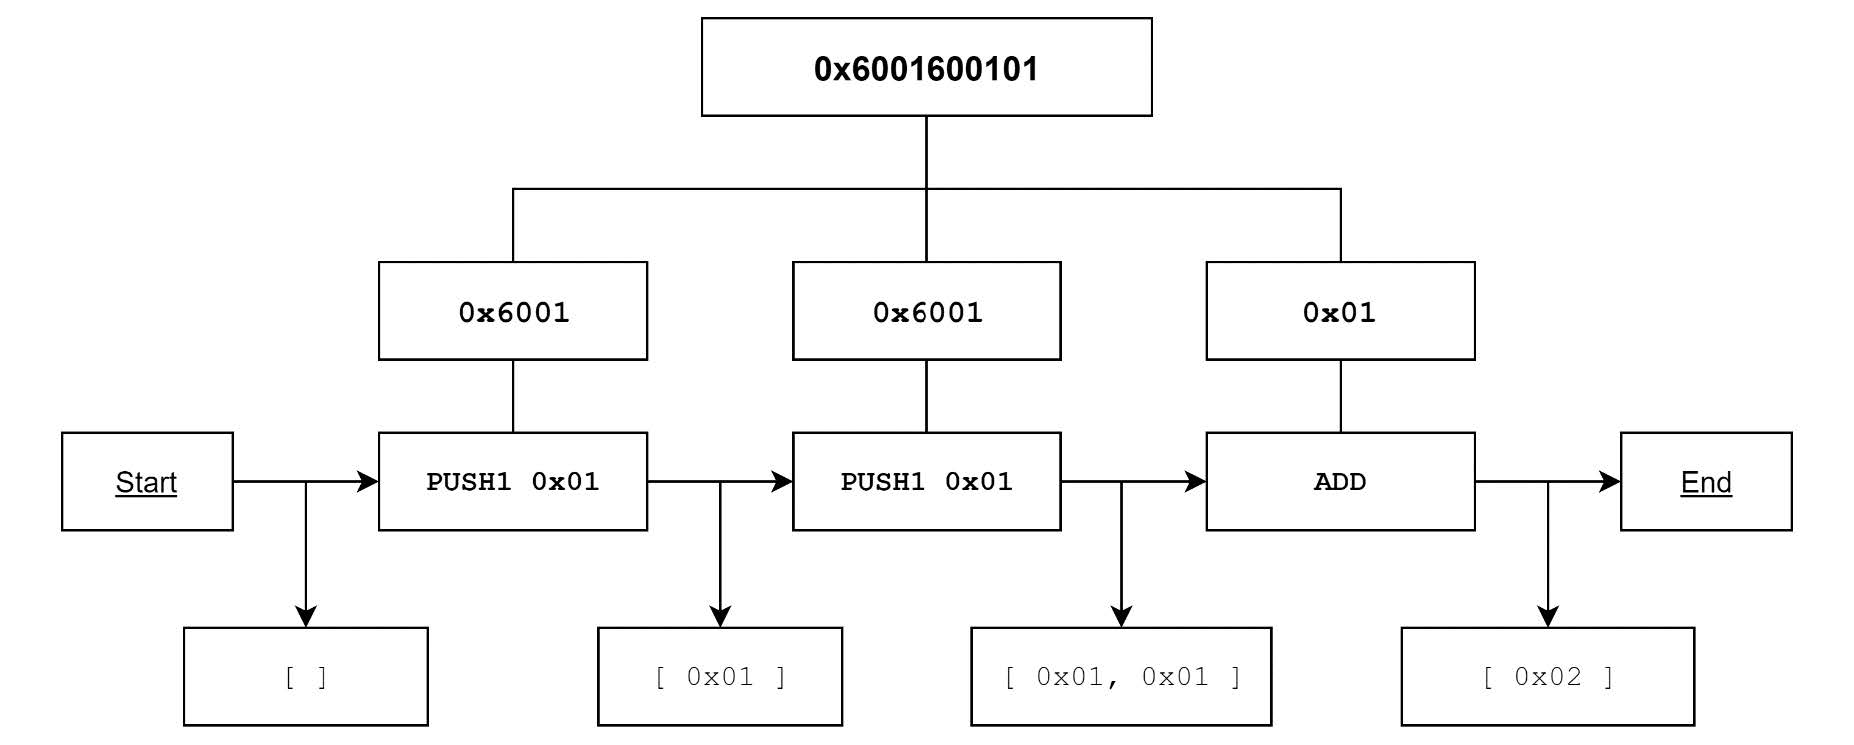
\includegraphics[width=\linewidth]{Images/Bytecode_example.jpg}
    \caption{Bytecode summing the values 1 and 1 -- The bottom row of blocks represents the stack.}
    \label{fig:bytecode}
\end{figure}

Consider the following bytecode, which adds the values 1 and 1.

\begin{itemize}
    \item \textbf{Bytecode:} \texttt{0x6001600101}
    
    \item \textbf{Code visual inspection:} The code can be broken down by analyzing the bytecode hexadecimal string two digits at a time (see figure \ref{fig:bytecode}).
    \begin{enumerate}
        \item \texttt{0x60 01} $\longrightarrow$ \texttt{PUSH1 0x01}
        \item \texttt{0x60 01} $\longrightarrow$ \texttt{PUSH1 0x01}
        \item \texttt{0x01} $\longrightarrow$ \texttt{ADD}
    \end{enumerate}
    
    \item
        \textbf{Disassembled Code:}
        \begin{lstlisting}
            00000: PUSH1 0x01
            00002: PUSH1 0x01
            00004: ADD
        \end{lstlisting}
\end{itemize}

\noindent
\textit{Note:} The program counter (PC, the number before the colon character) does not increase by a fixed amount. 
Instead, it advances by the number of bytes of the current instruction.
While most opcodes are 1 byte long, \texttt{PUSHn} instructions occupy \texttt{1 + n} bytes, since they include immediate data.\\

The execution trace proceeds as follows:

\begin{enumerate}
    \item The stack starts empty.
    \item The first \texttt{PUSH1} instruction places the value \texttt{0x01} onto the stack. The stack is now \texttt{[0x01]}.
    \item The second \texttt{PUSH1} instruction places another \texttt{0x01} onto the stack. The stack is now \texttt{[0x01, 0x01]}.
    \item The \texttt{ADD} instruction pops the top two items (\texttt{0x01} and \texttt{0x01}), adds them, and pushes the result (\texttt{0x02}) back onto the stack. The final stack is \texttt{[0x02]}.
\end{enumerate}

\subsection{Example 2: Storing and Returning a Value}

This example expands on the first by storing the result in memory and then returning it.

\begin{itemize}
    \item \textbf{Bytecode:} \texttt{0x60016001016000526001601ff3}

    \item \textbf{Code visual inspection:}
    \begin{enumerate}
        \item \texttt{0x60 01} $\longrightarrow$ \texttt{PUSH1 0x01}
        \item \texttt{0x60 01} $\longrightarrow$ \texttt{PUSH1 0x01}
        \item \texttt{0x01} $\longrightarrow$ \texttt{ADD}
        \item \texttt{0x60 00} $\longrightarrow$ \texttt{PUSH1 0x00}
        \item \texttt{0x52} $\longrightarrow$ \texttt{MSTORE}
        \item \texttt{0x60 01} $\longrightarrow$ \texttt{PUSH1 0x01}
        \item \texttt{0x60 1f} $\longrightarrow$ \texttt{PUSH1 0x1f}
        \item \texttt{0xf3} $\longrightarrow$ \texttt{RETURN}
    \end{enumerate}
    
    \item
        \textbf{Disassembled Code:}
        \begin{lstlisting}
            00000: PUSH1 0x01
            00002: PUSH1 0x01
            00004: ADD
            00005: PUSH1 0x00
            00007: MSTORE
            00008: PUSH1 0x01
            0000a: PUSH1 0x1f
            0000c: RETURN
        \end{lstlisting}
\end{itemize}

The execution trace is more complex:

\begin{enumerate}
    \item The first three instructions execute as before, leaving \texttt{[0x02]} on the stack.
    \item \texttt{PUSH1 0x00} pushes the value \texttt{0x00} onto the stack, which now holds \texttt{[0x00, 0x02]}.
    \item \texttt{MSTORE} pops the top two values. It uses \texttt{0x00} as the memory offset and \texttt{0x02} as the value to write. It stores \texttt{0x02} as a full 32-byte word at memory location 0.
    \item \texttt{PUSH1 0x01} pushes \texttt{0x01} onto the stack. This will be the size of the data to return.
    \item \texttt{PUSH1 0x1f} pushes \texttt{0x1f} (decimal 31) onto the stack. This will be the memory offset from which to read the return data. The stack now contains \texttt{[0x1f, 0x01]}.
    \item \texttt{RETURN} pops the offset (\texttt{0x1f}) and size (\texttt{0x01}). It reads 1 byte of data starting from memory offset 31. Because the value \texttt{0x02} was stored as a 32-byte word, the byte at this position is \texttt{0x02}. This value is returned as the result of the execution.
\end{enumerate}

\section{Practical execution of the previous examples}

\subsection{Environment setup}

To execute all the Ethereum operations on your machine you are highly encouraged to use a Linux distro inside a virtual machine in order to not interfere with your main host operating system. I use VirtualBox for the virtual machine generation and management and Ubuntu as the operating system of the virtual machine.\\

Inside the virtual machine, you need to install a C compiler (gcc is included in the \textbf{build-essential} package), the \textbf{Go language package} and \textbf{Ethereum Geth version 1.14} (the latest package does not have the same functionality required to run the examples).\\

\begin{lstlisting}[caption={Bash command to install the Geth requirements}]
    sudo apt install build-essential golang-go
\end{lstlisting}

To install an older version of Ethereum Geth you can follow this \href{https://medium.com/@jeffrey.kao.taipei/how-to-install-specific-older-version-etherium-geth-on-linux-3b9be9fed470}{guide}. I installed the version \textbf{Geth \& Tools 1.14.13}.\\

Once you installed everything, all you have to do is to create a folder to contain the two previously exposed examples.

\subsection{Decompilation and debug of example 1}

\begin{enumerate}
    \item
        Save the bytecode as text readable file:
        \begin{lstlisting}
            echo 6001600101 > sum.bc
        \end{lstlisting}

    \item
        Disassembly the code with the disasm tool of the EVM:
        \begin{lstlisting}
            evm disasm sum.bc
        \end{lstlisting}
        You will see the following result:
        \begin{lstlisting}
            6001600101
            00000: PUSH1 0x01
            00002: PUSH1 0x01
            00004: ADD
        \end{lstlisting}
        The first row is the bytecode contained in the file and the rest of the output is the decompiled code we derived after the visual inspection.

    \item 
        Run the code in debug mode:
        \begin{lstlisting}
            evm --debug --code 6001600101 run
        \end{lstlisting}
        You will see the following result:
        \begin{lstlisting}
            * BLANK LINE *
            #### TRACE ####
            PUSH1           pc=00000000 gas=10000000000 cost=3
            
            PUSH1           pc=00000002 gas=9999999997 cost=3
            Stack:
            00000000  0x1
            
            ADD             pc=00000004 gas=9999999994 cost=3
            Stack:
            00000000  0x1
            00000001  0x1
            
            STOP            pc=00000005 gas=9999999991 cost=0
            Stack:
            00000000  0x2
            
            #### LOGS ####
        \end{lstlisting}
        I have highlighted the fact that the first line is blank in the result because it's important to notice this detail. This is due to the fact that the considered program does not have a return statement so the output is null.\\

        The output contains all the steps described in the previous section in which we described the code.\\
        \noindent
        \textit{Note:} The lines below an instruction represent the state of the stack at the time of the execution of the command. This is the reason why there isn't a stack description below the first command and the reason why the stack description below the second \texttt{PUSH1} command contains only the number pushed in the stack by the first command.
\end{enumerate}

\subsection{Decompilation and debug of example 2}

\begin{enumerate}
    \item
        Save the bytecode as text readable file:
        \begin{lstlisting}
            echo 60016001016000526001601ff3 > sum2.bc
        \end{lstlisting}

    \item
        Disassembly the code with the disasm tool of the EVM:
        \begin{lstlisting}
            evm disasm sum2.bc
        \end{lstlisting}
        You will see the following result:
        \begin{lstlisting}
            60016001016000526001601ff3
            00000: PUSH1 0x01
            00002: PUSH1 0x01
            00004: ADD
            00005: PUSH1 0x00
            00007: MSTORE
            00008: PUSH1 0x01
            0000a: PUSH1 0x1f
            0000c: RETURN
        \end{lstlisting}
        The first row is the bytecode contained in the file and the rest of the output is the decompiled code we derived after the visual inspection.

    \item 
        Run the code in debug mode:
        \begin{lstlisting}
            evm --debug --code 60016001016000526001601ff3 run
        \end{lstlisting}
        You will see the following result:
        \begin{lstlisting}
            0x02
            #### TRACE ####
            PUSH1           pc=00000000 gas=10000000000 cost=3
            
            PUSH1           pc=00000002 gas=9999999997 cost=3
            Stack:
            00000000  0x1
            
            ADD             pc=00000004 gas=9999999994 cost=3
            Stack:
            00000000  0x1
            00000001  0x1
            
            PUSH1           pc=00000005 gas=9999999991 cost=3
            Stack:
            00000000  0x2
            
            MSTORE          pc=00000007 gas=9999999988 cost=6
            Stack:
            00000000  0x0
            00000001  0x2
            Memory:
            00000000  00 00 00 00 00 00 00 00  00 00 00 00 00 00 00 00
            00000010  00 00 00 00 00 00 00 00  00 00 00 00 00 00 00 00
            
            PUSH1           pc=00000008 gas=9999999982 cost=3
            Memory:
            00000000  00 00 00 00 00 00 00 00  00 00 00 00 00 00 00 00
            00000010  00 00 00 00 00 00 00 00  00 00 00 00 00 00 00 02
            
            PUSH1           pc=00000010 gas=9999999979 cost=3
            Stack:
            00000000  0x1
            Memory:
            00000000  00 00 00 00 00 00 00 00  00 00 00 00 00 00 00 00
            00000010  00 00 00 00 00 00 00 00  00 00 00 00 00 00 00 02
            
            RETURN          pc=00000012 gas=9999999976 cost=0
            Stack:
            00000000  0x1f
            00000001  0x1
            Memory:
            00000000  00 00 00 00 00 00 00 00  00 00 00 00 00 00 00 00
            00000010  00 00 00 00 00 00 00 00  00 00 00 00 00 00 00 02
            
            #### LOGS ####
        \end{lstlisting}
        In this case, the program has a return statement so the first line of the output is the value returned by the program. Like in the previous example, the rest of the output contains all the steps described in the previous section in which we described the code.\\

        \noindent
        \texttt{Note:} The output of the last command was edited to add the content of the contract memory. Unfortunately, it is not possible to show this information using more modern versions of Go and Gether. What really matters in this case is not the exact reproducibility of the experiment but understanding the process.\\

        I invite you to observe the representation of the memory: EVM uses a big-endian logic meaning that the most significant bit has a lower address than the others. This is the reason why the value \texttt{0x02} is stored at the very end of the 32-byte word. The memory is represented using 16-bytes rows with a double space between the 7th and the 8th byte for a more tidy representation. $(00000010)_{16}=(16)_{10}$. For this reason the offset of the second row is \texttt{00000010}.
\end{enumerate}

The Ethereum Virtual Machine, with its deterministic, gas-powered, and stack-based architecture, provides the secure and reliable foundation necessary for all smart contract functionality on the Ethereum network.

\end{document}
